%\documentclass[10pt,twocolumn,letterpaper,draft]{article}
\documentclass[10pt,letterpaper]{ctexart}

\usepackage{cvpr}
\usepackage{wrapfig}
\usepackage{graphicx}
\usepackage{amsmath}
\usepackage{amssymb}
\usepackage{booktabs}
\usepackage{subfigure}
\usepackage{algorithm}
\usepackage{algorithmicx}
\usepackage{algpseudocode}
\usepackage{listings}

\lstset{language=C++,
    basicstyle=\ttfamily,
    frame=single,
    keywordstyle=\color{blue}\ttfamily,
    stringstyle=\color{magenta}\ttfamily,
    commentstyle=\color{green}\ttfamily,
    morecomment=[l][\color{magenta}]{\#},
    morekeywords={*,size_t,cudaEvent_t },
}

\renewcommand{\labelenumi}{\alph{enumi}.} % Make numbering in the enumerate environment by letter rather than number (e.g. section 6)
\floatname{algorithm}{算法}
\renewcommand{\algorithmicrequire}{\textbf{输入:}}
\renewcommand{\algorithmicensure}{\textbf{输出:}}
\renewcommand{\lstlistingname}{代码清单}

\usepackage{enumitem}
\setenumerate[1]{itemsep=0pt,partopsep=0pt,parsep=\parskip,topsep=5pt}
\setitemize[1]{itemsep=0pt,partopsep=0pt,parsep=\parskip,topsep=5pt}
\setdescription{itemsep=0pt,partopsep=0pt,parsep=\parskip,topsep=5pt}

% Include other packages here, before hyperref.

% If you comment hyperref and then uncomment it, you should delete
% egpaper.aux before re-running latex.  (Or just hit 'q' on the first latex
% run, let it finish, and you should be clear).
\usepackage[pagebackref=true,breaklinks=true,letterpaper=true,colorlinks,bookmarks=false]{hyperref}


\cvprfinalcopy % *** Uncomment this line for the final submission

\def\cvprPaperID{159} % *** Enter the CVPR Paper ID here
\def\httilde{\mbox{\tt\raisebox{-.5ex}{\symbol{126}}}}

\newcommand{\mypara}[1]{\paragraph{#1.}}

\graphicspath{{figures/}}

% Pages are numbered in submission mode, and unnumbered in camera-ready
%\ifcvprfinal\pagestyle{empty}\fi
\setcounter{page}{1}


%\begin{CJK*}{GBK}{song}

\newcommand{\figref}[1]{图\ref{#1}}
\newcommand{\tabref}[1]{表\ref{#1}}
\newcommand{\equref}[1]{式\ref{#1}}
\newcommand{\secref}[1]{第\ref{#1}节}

\ctexset{
  section={
    number={\chinese{section}},
    format={\heiti},
    beforeskip={0.1ex},
    afterskip={0.1ex},
    indent={\parindent},
    },
}
\usepackage{zhnumber}

\newcommand\zhsubsec[1]{{% 中文小节
\bfseries{
\stepcounter{subsection}(\zhnum{subsection}){#1}}
\vspace{0.1pt}%
}}

%%%%%%%%% TITLE
\begin{document}
\pagestyle{plain}
\title{
    \begin{center}
        \phantom{Start!}
        \vspace{2cm}
        \center{\zihao{1} 中山大学数据科学与计算机学院}
        \center{\zihao{2} 《高性能程序设计基础》实验7}
        \center{(2018-2019学年秋季学期)}
    \end{center}
}
\maketitle

\begin{center}
    \setlength{\baselineskip}{40pt}
    \vspace{1cm}
    \zihao{-2}
    \center{
        \begin{tabular}{cc}
        学\qquad 号:& \underline{~~~~~~16337113~~~~~~}  \\
        姓\qquad 名:& \underline{~~~~~~~劳马东~~~~~~~}  \\
        教学班级:   & \underline{~~~~~教务2班~~~~~}  \\
        专\qquad 业:& \underline{~~~~~~~~~超算~~~~~~~~}  \\
       \end{tabular}
    }
\end{center}
\pagebreak

%%%%%%%%% BODY TEXT %%%%%%%%%%%%




% \begin{figure}[h]
%   \centering
%   \subfigure[Completeness]{
%   \includegraphics[width=0.4\textwidth]{dfs-1.png}
%   \label{fig:dfs-1}}
% \end{figure}

\section{实验题目}
\begin{enumerate}[itemindent=2em,label=\arabic*、]
\item 完成cuda的“Hello world”程序,编译运行grid=(2,4),block=(8,16),给出输出结果文件。

\item 完成CUDA的两个矩阵乘法A*B=C,其中A,B是5000*5000的方阵。假设矩阵A的元素为aij=i-0.1*j+1,矩阵B的元素为bij=0.2*j-0.1*i。
\end{enumerate}

\section{实验过程}

\zhsubsec{一些约定}
\par 假设A、B矩阵是$WIDTH \times WIDTH$矩阵:
\begin{enumerate}[itemindent=2em,label=\arabic*、]
    \item grid和block都是二维方阵,grid的大小为$M \times M$, block大小为$N \times N$;
    \item $\frac{WIDTH}{M \times N}$是整数;
    \item 一个block最多有512个线程 $\Rightarrow N \leq \lfloor \sqrt{512} \rfloor = 20$;
\end{enumerate}

\zhsubsec{矩阵分块}

在\_\_global\_\_函数中,我们能够得到一个线程的$blockIdx$和$threadIdx$,如何根据这两个坐标,找到线程对应的子矩阵呢?
在CUDA中,线程的分布情况如\figref{fig:block-thread}。一个grid中有多个block,它的$blockIdx$中的$(x,y)$表示它的坐标,
而不是行列号;同理,一个block中有多个thread,它的$threadIdx$同样是坐标。例如,在\figref{fig:block-thread}中,绿色
表示一个grid,$(0,0)$ block右边是$(1,0)$ block,下面是$(0, 1)$ block;橙色表示一个block,$(0,0$ thread右边是
$(1,0)$ thread,下面是$(0,1)$ thread。
\par 基于线程分布,我们就可以将坐标相同的线程与矩阵块对应起来,如\figref{fig:divide},上半部分每一个橙色的小格是一个线程,
下半部分每一个灰色的小格是矩阵的一个块(不一定是$1\times 1$)。
\begin{figure}[H]
    \centering
    \subfigure[CUDA中的线程层次]{
        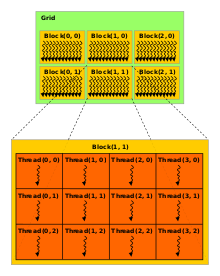
\includegraphics[width=0.4\textwidth]{block-thread.png}
        \label{fig:block-thread}
    }
    \subfigure[矩阵分块示意图]{
        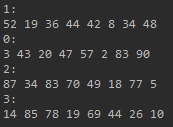
\includegraphics[width=0.32\textwidth]{divide.png}
        \label{fig:divide}
    }
\end{figure}
如此,一个线程对应的矩阵块的起始$(i, j)$可以这样计算(这里的$i$、$j$是绝对而不是相对):
\begin{equation}
    \begin{aligned}
        &block\_i = blockIdx.y \times \frac{WIDTH}{gridDim.x}\\
        &block\_j = blockIdx.x \times \frac{WIDTH}{gridDim.x}\\
        &i = block\_i + threadIdx.y \times \frac{WIDTH}{gridDim.x \times blockDim.x}\\
        &j = block\_j + threadIdx.x \times \frac{WIDTH}{gridDim.x \times blockDim.x}\\
    \end{aligned}
\end{equation}

\zhsubsec{子矩阵乘法}
\par 在这里,子矩阵乘法并不是线性代数中矩阵分块乘法。由于线程之间不涉及通信,每个线程需要计算它对应的结果子矩阵的每个元素的最终结果。
因此,为了计算结果矩阵$(i, j)$位的一个元素,一个线程需要遍历矩阵A的第$i$行的所有元素和矩阵B第$j$列的所有元素,即。
\begin{algorithm}
    \caption{线程计算其结果子矩阵}
    \begin{algorithmic}[1] %每行显示行号
        \Require 线程的矩阵块的全局起始行列号$(i, j)$,输入矩阵$A$、$B$,结果矩阵$C$
        \Function {$thread\_matrix\_mul$}{$i, j, A, B, C$}
            \State $local\_width \gets \frac{WIDTH}{gridDim.x \times blockDim.x}$
            \For {$local\_i \in [0, local\_width)$}
                \State $global\_i \gets i + local\_i$ 
                \For{$local\_j \in [0, local\_width)$}
                    \State $global\_j \gets j + local\_j$
                    \State $sum \gets 0$
                    \For{$k \in [0, WIDTH)$}
                        \State $sum \gets sum + A[global\_i][k] * B[k][global\_j]$
                    \EndFor
                    \State store $sum$ to $C[global\_i][global\_j]$
                \EndFor
            \EndFor
        \EndFunction
    \end{algorithmic}
\end{algorithm}

\section{关键代码}
\begin{enumerate}[itemindent=2em, label=\arabic*、]
    \item 矩阵分块
\begin{lstlisting}[caption=矩阵分块,captionpos=b]
__global__ void matrix_mul_kernel(double* P, unsigned n) {
    size_t n_per_block = n/gridDim.x, n_per_thread = n_per_block/blockDim.x;
    size_t block_i = blockIdx.y*n_per_block, block_j = blockIdx.x*n_per_block;
    size_t thread_i = block_i + threadIdx.y * n_per_thread,
           thread_j = block_j + threadIdx.x * n_per_thread;
    ...
}
\end{lstlisting}
    \item 子矩阵乘法
\begin{lstlisting}[caption=计算结果矩阵,captionpos=b]
__device__ void cal_one_ele(size_t i, size_t j, size_t n, double* P) {
    double sum = 0;
    for (int k = 0; k < n; ++k) {
        double a_ik = i - 0.1 * k + 1, b_kj = 0.2 * j - 0.1 * k;
        sum += a_ik * b_kj;
    }
    *(P + i * n + j) = sum;
}
__global__ void matrix_mul_kernel(double* P, unsigned n) {
    ...
    for (int i = 0; i < n_per_thread; ++i) {
        size_t ii = thread_i + i;
        for (int j = 0; j < n_per_thread; ++j) {
            cal_one_ele(ii, thread_j + j, n, P);
        }
    }
}
\end{lstlisting}    
    \item 统计GPU时间
    \par \qquad 在并行程序中,想要统计程序整体的运行时间,就需要在计时前做同步。在MPI中,提供了Barrier机制实现同步,类似的,CUDA有事件同步。
    在开始调用核函数之前,让时间记录下时间点,程序运行完成后,使用cudaEventSynchronize函数同步,记录此时的时间点。两次事件记录之间
    的时间差计时核函数运行的时间,可用cudaEventElapsedTime获得。值得一提的是,直接使用clock函数统计得到的是CPU的运行时间,因为CPU调用完核函数后,
    并不等待其运行完成,直接就返回了。
\begin{lstlisting}[caption=用事件统计程序运行时间,captionpos=b]
    float elapsed=0;
    cudaEvent_t start, stop;
    cudaEventCreate(&start);
    cudaEventCreate(&stop);

    cudaEventRecord(start, nullptr);

    matrix_mul_kernel<<<grid_dim, block_dim>>>(result.data().get(), n);

    cudaEventRecord(stop, nullptr);
    cudaEventSynchronize (stop);
    cudaEventElapsedTime(&elapsed, start, stop);
    cudaEventDestroy(start);
    cudaEventDestroy(stop);
\end{lstlisting}

\end{enumerate}
\section{实验结果及分析}
实验平台为Google Colab(GPU Tesla K80),测得串行代码矩阵相乘部分的时间是1882.77秒;使用sm\_30架构,并行时间如下。
\begin{table}[!htbp]
    \centering
    \begin{tabular}{cc|cc}
        \toprule
        grid & block & kernel时间/s & 加速比\\
        \hline
        $250 \times 250$ & $20 \times 20$ & 1.27853 & 1472.6\\
        $125 \times 125$ & $20 \times 20$ & 1.25271 & 1502.9\\
        $500 \times 500$ & $10 \times 10$ & 1.37771 & 1366.6\\
        $1000 \times 1000$ & $10 \times 10$ & 1.64177 & 1146.8\\
        \bottomrule
    \end{tabular}
\end{table}
\end{document}
